%\documentclass[12pt,notitlepage]{article}
\documentclass[a4paper,12pt]{article}
\usepackage[utf8]{inputenc}
\usepackage{graphicx}
\usepackage{verbatim}
\usepackage{amsthm}
\usepackage{amssymb}
\usepackage{pdfpages}
\usepackage{amsmath}
\usepackage{tikzsymbols}
\usepackage{mwe}
\usetikzlibrary{decorations.pathreplacing}
\usetikzlibrary{shapes}
\usepackage{mathtools}
\usepackage{enumitem}
\DeclarePairedDelimiter\ceil{\lceil}{\rceil}
\DeclarePairedDelimiter\floor{\lfloor}{\rfloor}

\usepackage{hyperref}
%\usepackage[T1]{fontenc}
\usepackage{url}
\usepackage{lipsum}
\usepackage{array}
\usepackage{multirow}
\usepackage{float}
\usepackage{lscape}
\usepackage{colortbl}
\newcolumntype{P}[1]{>{\centering\arraybackslash}p{#1}}
\usepackage[nottoc,numbib]{tocbibind}
\usepackage{fancyhdr}
\usepackage{hhline}
\usepackage[printonlyused]{acronym}

%\usepackage{txfonts}
\usepackage{lipsum,etoolbox}% http://ctan.org/pkg/{lipsum,etoolbox}
\usepackage{caption}
\usepackage{subcaption}

\usepackage{algorithm}
\usepackage[noend]{algpseudocode}

\makeatletter
\def\BState{\State\hskip-\ALG@thistlm}
\makeatother

\usepackage{minted}

\definecolor{black}{RGB}{0,0,0}

\usepackage{fancyvrb}

\usepackage{geometry}
\geometry{
	a4paper,
	total={170mm,257mm},
	right=3cm,
	left=3.5cm,
	top=3cm,
	bottom=3cm
}

\makeatletter
\DeclareRobustCommand{\rvdots}{%
	\vbox{
		\baselineskip4\p@\lineskiplimit\z@
		\kern-\p@
		\hbox{.}\hbox{.}\hbox{.}
}}
\makeatother
\usepackage{titlesec}
\usepackage{hyperref}
\titleclass{\subsubsubsection}{straight}[\subsection]

\newcounter{subsubsubsection}[subsubsection]
\renewcommand\thesubsubsubsection{\thesubsubsection.\arabic{subsubsubsection}}
\renewcommand\theparagraph{\thesubsubsubsection.\arabic{paragraph}} % optional; useful if paragraphs are to be numbered

\titleformat{\subsubsubsection}
{\normalfont\normalsize\bfseries}{\thesubsubsubsection}{1em}{}
\titlespacing*{\subsubsubsection}
{0pt}{3.25ex plus 1ex minus .2ex}{1.5ex plus .2ex}

\makeatletter
\renewcommand\paragraph{\@startsection{paragraph}{5}{\z@}%
	{3.25ex \@plus1ex \@minus.2ex}%
	{-1em}%
	{\normalfont\normalsize\bfseries}}
\renewcommand\subparagraph{\@startsection{subparagraph}{6}{\parindent}%
	{3.25ex \@plus1ex \@minus .2ex}%
	{-1em}%
	{\normalfont\normalsize\bfseries}}
\def\toclevel@subsubsubsection{4}
\def\toclevel@paragraph{5}
\def\toclevel@paragraph{6}
\def\l@subsubsubsection{\@dottedtocline{4}{7em}{4em}}
\def\l@paragraph{\@dottedtocline{5}{10em}{5em}}
\def\l@subparagraph{\@dottedtocline{6}{14em}{6em}}
\makeatother
\newcommand*\circled[1]{\tikz[baseline=(char.base)]{
		\node[shape=circle,draw,inner sep=2pt] (char) {#1};}}


\setcounter{secnumdepth}{4}
\setcounter{tocdepth}{4}
\newcommand{\und}{\underline{\hspace{.10in}}}
\begin{document}
	\begin{titlepage}
		\begin{center}
			\vspace*{9em}
			\Huge 
			MH4921\\ Supervised Independent Study II\\
			\vspace*{4em}
			\LARGE
			\textbf{Local DNS Attack}\\		
			\vspace{4em}
			\textbf{Brandon Goh Wen Heng}\\
			\vspace*{4em}
			Academic Year 2018/19
			\vfill
		\end{center}
	\end{titlepage}
	
	\pagenumbering{roman}
	\tableofcontents
	\newpage
	\pagenumbering{arabic}
	\section{Introduction}
	The Domain Name System (DNS) is used to translate hostnames to IP addresses. This process is termed as DNS resolution, which is transparent to users. However, there are attacks that can be mounted against the DNS resolution process which can redirect the user away from a legitimate to a malicious site, also known as DNS Pharming attacks.
\section{Overview}
This lab will focus on the effects of the HOSTS file on the redirection of any request, manipulation of the DNS cache of both on the user's system in the second task and on the DNS server in the third task as a more effective measure. Using any of the three attacks will render the user vulnerable, with the potential of exposing this to a greater number of systems if it was performed on a DNS server such as an Internet Service Provider (ISP) and was successful.
\newpage
\section{Attack Sequence}
\subsection{Virtual Machine (VM) Preparation}
\subsubsection{Network Setup}\begin{par}
In the following lab, 3 VMs are configured in the layout shown in Figure \ref{fig:Networksetup}. The figure also displays how a local network is connected to the wider internet and how domains are resolved.\end{par}
\begin{figure}[H]
			\centering
			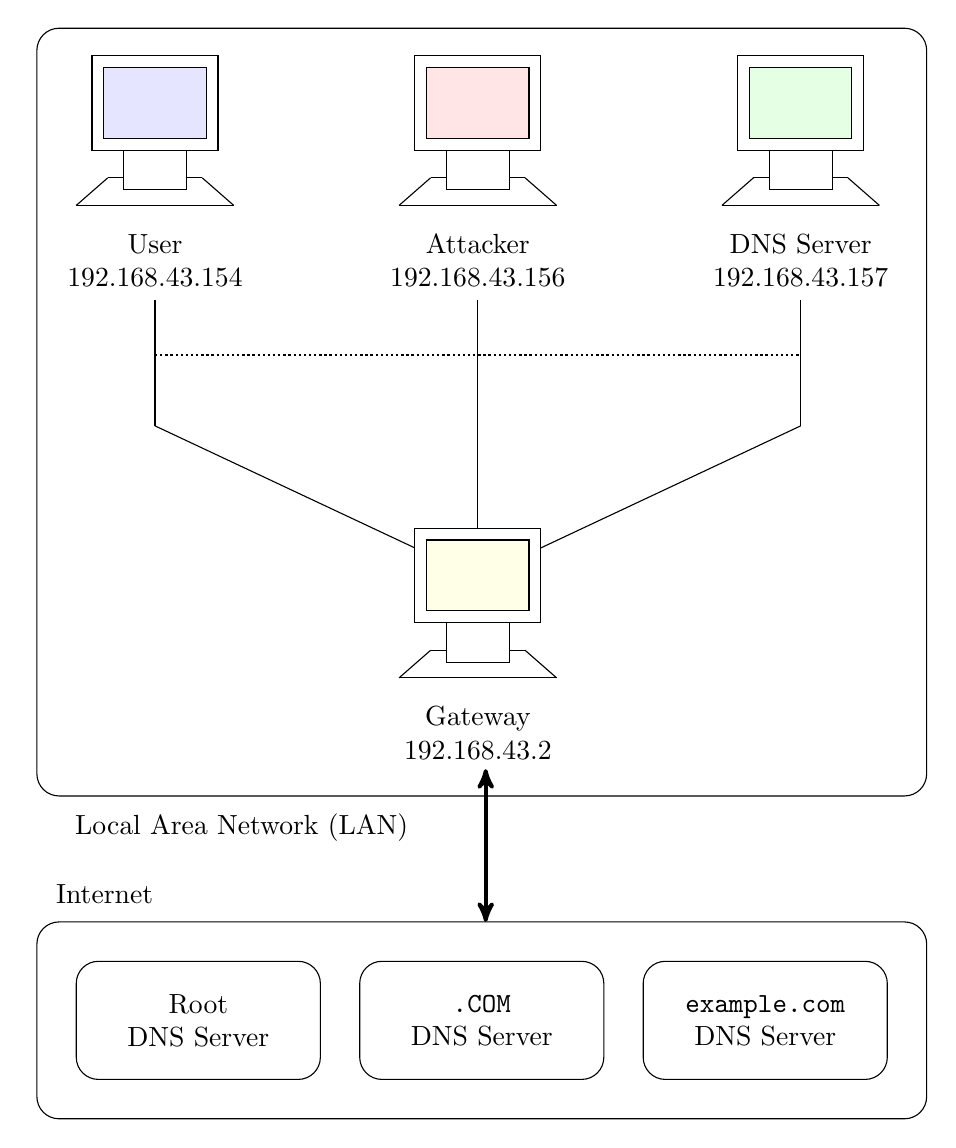
\begin{tikzpicture}
			\draw[fill=red!10] (-1.05,2.15) rectangle (0.25,1.25);
			\draw (-1.2,2.3) rectangle (0.4,1.1);
			\draw (0,1.1) rectangle (-0.8,0.6);
			\draw (-1,0.75) -- (-1.4,0.4);
			\draw (0.2,0.75) -- (0.6,0.4);
			\draw (-1.4,0.4) -- (0.6,0.4);
			\draw (-1,0.75) -- (-0.8,0.75);
			\draw (0.2,0.75) -- (0,0.75);
			\draw (-0.4,-0.3) node[text width=3cm,align=center]{Attacker\\192.168.43.156};
			
			
			\draw[fill=blue!10] (-5.15,2.15) rectangle (-3.85,1.25);
			\draw (-5.3,2.3) rectangle (-3.7,1.1);
			\draw (-4.1,1.1) rectangle (-4.9,0.6);
			\draw (-5.1,0.75) -- (-5.5,0.4);
			\draw (-3.9,0.75) -- (-3.5,0.4);
			\draw (-5.5,0.4) -- (-3.5,0.4);
			\draw (-5.1,0.75) -- (-4.9,0.75);
			\draw (-3.9,0.75) -- (-4.1,0.75);
			\draw (-4.5,-0.3) node[text width=3cm, align=center]{User\\192.168.43.154};
			
				\draw[fill=green!10] (3.05,2.15) rectangle (4.35,1.25);
			\draw (2.9,2.3) rectangle (4.5,1.1);
			\draw (4.1,1.1) rectangle (3.3,0.6);
			\draw (3.1,0.75) -- (2.7,0.4);
			\draw (4.3,0.75) -- (4.7,0.4);
			\draw (2.7,0.4) -- (4.7,0.4);
			\draw (3.1,0.75) -- (3.3,0.75);
			\draw (4.3,0.75) -- (4.1,0.75);
			\draw (3.7 ,-0.3) node[text width=3cm, align=center]{DNS Server\\192.168.43.157};
			
			\draw (3.7,-0.8) -- (3.7,-2.4);
			\draw (-4.5,-0.8) -- (-4.5,-2.4);
			\draw (-0.4,-0.8) -- (-0.4,-3.7);
			\draw (3.7,-2.4) -- (0.4,-3.95);
			\draw (-4.5,-2.4)--(-1.2,-3.95);
			\draw[densely dotted, line width=0.3mm](-4.5,-1.5) -- (3.7,-1.5);
			
			
			\draw[fill=yellow!10] (-1.05,-3.85) rectangle (0.25,-4.75);
			\draw (-1.2,-3.7) rectangle (0.4,-4.9);
			\draw (0,-4.9) rectangle (-0.8,-5.4);
			\draw (-1,-5.25) -- (-1.4,-5.6);
			\draw (0.2,-5.25) -- (0.6,-5.6);
			\draw (-1.4,-5.6) -- (0.6,-5.6);
			\draw (-1,-5.25) -- (-0.8,-5.25);
			\draw (0.2,-5.25) -- (0,-5.25);
			\draw (-0.4,-6.3) node[text width=3cm,align=center]{Gateway\\192.168.43.2};
			
			\draw[rounded corners=8pt] (-6,2.65) rectangle (5.3,-7.1);
			
			\draw[<->,>=stealth',line width=0.5mm] (-0.3,-6.76) -- (-0.3, -8.7);
			
			\draw[rounded corners=8pt] (-6,-8.7) rectangle (5.3,-11.2);
			
			\draw (-3.4,-7.5) node[align=left]{Local Area Network (LAN)};
			\draw (-5.14,-8.35) node[align=left]{Internet};
			
			\draw [rounded corners=8pt] (-5.5,-9.2) rectangle node[text width=3cm, align=center]{Root\\DNS Server} (-2.4, -10.7);
			\draw [rounded corners=8pt] (-1.9,-9.2) rectangle node[text width=3cm, align=center]{\texttt{.COM}\\DNS Server} (1.2, -10.7);
			\draw [rounded corners=8pt] (1.7,-9.2) rectangle node[text width=3cm, align=center]{\texttt{example.com}\\DNS Server} (4.8, -10.7);
				\end{tikzpicture}
			\caption{Network Topology}
			\label{fig:Networksetup}
		\end{figure}
		\subsubsection{Installing DNS server}
		\begin{par} The DNS server that will be used on Ubuntu is \texttt{BIND9} and can be installed using the following line.
		\end{par}
		\begin{verbatim}
		$ sudo apt-get install bind9
		\end{verbatim}
		\subsubsection{Creating domain configuration files}
		\begin{par}
		For the DNS server to function, the configuration file \texttt{named.conf} needs to be present and reads additional files such as \texttt{named.conf.options}, all located in the folder \texttt{/etc/bind/}. The following lines are added so that the DNS server's cache dump can be read.
		\end{par}
		\begin{verbatim}
		options {
		    dump-file    "/var/cache/bind/dump.db";
		};
		\end{verbatim}
		\subsubsection{Creating zones}
		\begin{par} Each domain to be used on the server requires a zone file. This file provides answers on the domain that is being queried, in this lab \texttt{example.com}. The domain \texttt{example.com} is used to provide illustrative examples in documents and has no ownership, hence safe to us for this lab. The following lines are added to the file \texttt{/etc/bind/named.conf}.
		\end{par}
		\begin{verbatim}
		zone "example.com" {
		    type master;
		    file "/var/cache/bind/example.com.db";
		    };
		    
		zone "43.168.192.in-addr.arpa" {
		    type master;
		    file "/var/cache/bind/192.168.43";
		    };
		\end{verbatim}
		*Note: \texttt{in-addr.arpa} is used for the reverse mapping of IP addresses to hostnames and hence requires IP address to be specified in reverse order when declaring zones.
		\subsubsection{Setting up zone files}
		\begin{par}
		Zone files are required for DNS resolution to the respective domain names. Each zone  contains resource records which must contain a Start of Authority (SOA) record and followed with additional options such as Address (A) record, which specifies the IP\textbf{v4} address where this domain is located on. Other records that are mainly specified include NameServer (NS), Mail eXchange (MX), TeXT (TXT) records. There are instances where other records which are not mandatory that may appear, such as AAAA and CNAME records. The full list of records can be found on \href{https://www.iana.org/assignments/dns-parameters/dns-parameters.xhtml}{IANA's page}.\\\\The following zone files is used to configure \texttt{example.com}
		\end{par}
		\begin{verbatim}
		$TTL 3D
		@        IN    SOA    ns.example.com. admin.example.com. (
		         2008111001 ;serial, today's date + today's serial number
		         8H         ;refresh, seconds
		         2H         ;retry, seconds
		         4W         ;expire, seconds
		         1D)        ;minimum, seconds
		
		@        IN    NS    ns.example.com. ; Address of nameserver
		@        IN    MX    10 mail.example.com. ;Primary Mail Exchanger
		
		www      IN    A     192.168.43.101 ;Address of www.example.com
		mail     IN    A     192.168.43.102 ;Address of mail.example.com
		ns       IN    A     192.168.43.157 ;Address of ns.example.com
		*.example.com  IN  A 192.168.13.100 ;Address for other URL in 
		                                    ;example.com. domain
		\end{verbatim}
		A reverse DNS lookup file is also needed for IP address zone 192.168.43 for \texttt{example.com}
		\begin{verbatim}
		$TTL 3D
		@        IN    SOA    ns.example.com. admin.example.com. (
		               2008111001
		               8H
		               2H
		               4W
		               1D)
		@        IN    NS    ns.example.com.
		101      IN    PTR   www.example.com.
		102      IN    PTR   mail.example.com.
		10       IN    PTR   ns.example.com.
		\end{verbatim}
		\subsubsection{Starting the DNS server}
		To start the \texttt{BIND9} DNS server, the following command is executed in Terminal.
		\begin{verbatim}
		$sudo service bind9 restart
		\end{verbatim}
		\subsubsection{Configuring User Machine}
		\begin{par}
		On the user's machine, the default DNS server needs to be amended. This is done by changing the \texttt{resolv.conf} file. The following single line is added to the file.\end{par} 
		\begin{verbatim}
		nameserver 192.168.43.157 #IP address of server just setup
		\end{verbatim}
		\begin{par}
		Additionally, the changes made might be overwritten by the DHCP client and needs to be avoided to complete the lab properly. To do so, the DNS server address on our wired connection (Under IPv4 settings) is manually and explicitly defined. To refresh the connection and ensure that the changes take effect immediately, the name of our connection ``Wired connection 1" is clicked to force refresh the network.
		\end{par}
		\subsubsection{Checking of Output}
		\begin{par}
		To check if the server and the user has been configured correctly. The command \texttt{dig} is used to obtain information about the domain when a domain query has been issued to the DNS nameserver.
		\begin{verbatim}
		$ dig example.com
		\end{verbatim}
		The output will display common details such as the IP address of the domain and nameserver and TTL (Time-To-Live) of the DNS server.
		
\begin{figure}[H]
\centering
\includegraphics[width=0.85\linewidth]{dig}
\caption{Expected Output of DNS Server}
\label{fig:dig}
\end{figure}
		\end{par}
		\newpage
		\subsection{System Compromised}
		\begin{par}Assuming that the attackers have gained control over the system, this task will focus on the modification of the HOSTS file. Using the HOSTS file for hostname redirection ignores any DNS lookups. For this task, \texttt{example.com} has been redirected to some random IP address. From Figure \ref{fig:dig}, it is known that the site \texttt{www.example.com} has IP address 192.168.43.101 and can be checked by running the command \texttt{ping www.example.com}. \\\\The IP address is modified to reflect 1.2.3.4 in the HOSTS file, located at the directory \texttt{/etc/hosts} and pinged to show the effect.\end{par}
		\begin{figure}[H]
		    \centering
		    \begin{subfigure}[h]{0.49\textwidth}
		        \centering
		        \includegraphics[width=1\linewidth]{beforehost}
		        \caption{Before HOSTS Edit}
		    \end{subfigure}%
		    ~ 
		    \begin{subfigure}[h]{0.49\textwidth}
		        \centering
		        \includegraphics[width=1\linewidth]{afterhost}
		        \caption{After HOSTS Edit}
		    \end{subfigure}
		    \caption{Effect on HOSTS Edit}
		    \label{fig:hostsfile}
		\end{figure}
		\vspace{1em}
		\begin{par}
		\noindent As shown in Figure \ref{fig:hostsfile}, any entry in the HOSTS file takes precedence over the DNS lookup via the DNS server any attempt to establish a connection to an affected domain will result in a redirection that the user may not be aware if an attacker has modified the system.
		\end{par}
		\subsection{Spoofing User Response}
		\begin{par}
		For this section, the user's system is not compromised by the attacker. However, attackers will still be able to listen to the network and spoof a DNS request issued by the user. By this method, the system will acknowledge the fake DNS response and be redirected to the malicious domain. Figure \ref{fig:SpoofUserRes} provides a graphical overview on the flow of the DNS spoofing attack.
		
		\begin{figure}[H]
					\centering
					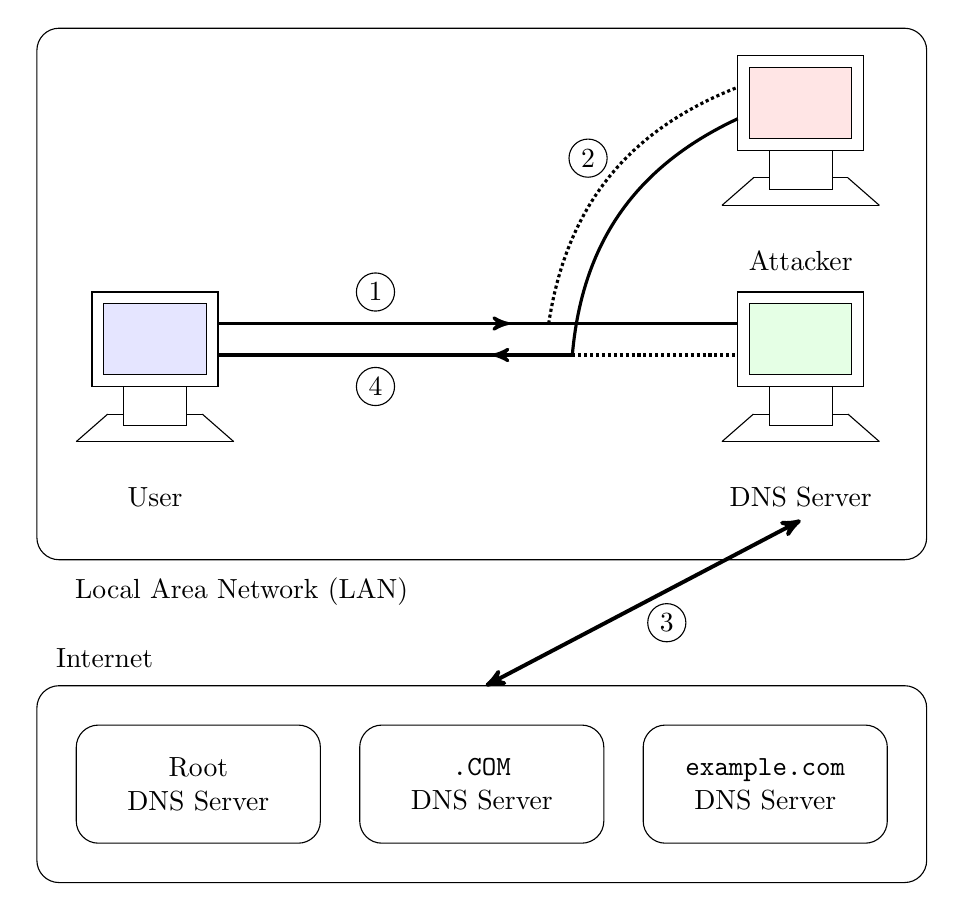
\begin{tikzpicture}
					\draw[fill=green!10] (3.05,-0.85) rectangle (4.35,-1.75);
					\draw (2.9,-0.7) rectangle (4.5,-1.9);
					\draw (4.1,-1.9) rectangle (3.3,-2.4);
					\draw (3.1,-2.25) -- (2.7,-2.6);
					\draw (4.3,-2.25) -- (4.7,-2.6);
					\draw (2.7,-2.6) -- (4.7,-2.6);
					\draw (3.1,-2.25) -- (3.3,-2.25);
					\draw (4.3,-2.25) -- (4.1,-2.25);
					\draw (3.7 ,-3.3) node[text width=3cm,align=center]{DNS Server};
					
					
					\draw[fill=blue!10] (-5.15,-0.85) rectangle (-3.85,-1.75);
					\draw (-5.3,-0.7) rectangle (-3.7,-1.9);
					\draw (-4.1,-1.9) rectangle (-4.9,-2.4);
					\draw (-5.1,-2.25) -- (-5.5,-2.6);
					\draw (-3.9,-2.25) -- (-3.5,-2.6);
					\draw (-5.5,-2.6) -- (-3.5,-2.6);
					\draw (-5.1,-2.25) -- (-4.9,-2.25);
					\draw (-3.9,-2.25) -- (-4.1,-2.25);
					\draw (-4.5,-3.3) node[text width=3cm, align=center]{User};
					
						\draw[fill=red!10] (3.05,2.15) rectangle (4.35,1.25);
					\draw (2.9,2.3) rectangle (4.5,1.1);
					\draw (4.1,1.1) rectangle (3.3,0.6);
					\draw (3.1,0.75) -- (2.7,0.4);
					\draw (4.3,0.75) -- (4.7,0.4);
					\draw (2.7,0.4) -- (4.7,0.4);
					\draw (3.1,0.75) -- (3.3,0.75);
					\draw (4.3,0.75) -- (4.1,0.75);
					\draw (3.7 ,-0.3) node[text width=3cm, align=center]{Attacker};
					
					\draw[rounded corners=8pt] (-6,2.65) rectangle (5.3,-4.1);
					
					\draw[<->,>=stealth',line width=0.5mm] (3.7,-3.6) -- (-0.3, -5.7);
					
					\draw[rounded corners=8pt] (-6,-5.7) rectangle (5.3,-8.2);
					
					\draw (-3.4,-4.5) node[align=left]{Local Area Network (LAN)};
					\draw (-5.14,-5.35) node[align=left]{Internet};
					
					\draw [rounded corners=8pt] (-5.5,-6.2) rectangle node[text width=3cm, align=center]{Root\\DNS Server} (-2.4, -7.7);
					\draw [rounded corners=8pt] (-1.9,-6.2) rectangle node[text width=3cm, align=center]{\texttt{.COM}\\DNS Server} (1.2, -7.7);
					\draw [rounded corners=8pt] (1.7,-6.2) rectangle node[text width=3cm, align=center]{\texttt{example.com}\\DNS Server} (4.8, -7.7);
					
					\draw[->,>=stealth',line width=0.4mm](-3.7,-1.1) --(0,-1.1);
					\draw[line width=0.4mm] (-0.3,-1.1)--(2.9,-1.1);
					\draw[bend left, line width=0.4mm, densely dotted] (0.5,-1.1) to (2.9,1.9);
					\draw[-<,>=stealth',line width=0.4mm](-3.7,-1.5) --(0,-1.5);
					\draw[line width=0.4mm](-0.1,-1.5) --(0.8,-1.5);
					\draw[line width=0.4mm, densely dotted] (0.8,-1.5)--(2.9,-1.5);
					\draw[bend left, line width=0.4mm] (0.8,-1.5) to (2.9,1.5);
					\draw (-1.7,-0.7) node{\circled{1}};
					\draw (2,-4.9) node{\circled{3}};
					\draw (1,1) node{\circled{2}};
					\draw (-1.7,-1.9) node {\circled{4}};
					\end{tikzpicture}
					
					\begin{flushleft}
					\circled{1} User's system sends out a DNS query to the DNS server.\\
					\circled{2} The attacker listens on the DNS request from the network and processes it.\\
					\circled{3} The DNS server will query other DNS servers if the records are not cached on the server.\\
					\circled{4} Before the DNS server is able to reply, the attacker sends out its own packet to respond to the user's DNS request and spoof the DNS cache on the user's system.
					\end{flushleft}
					\centering
					
					\caption{User DNS Spoofing}
					\label{fig:SpoofUserRes}
				\end{figure}
		
		
		\noindent For a DNS response to be accepted, the following criterion must be met:\end{par}
		\begin{enumerate}
		\itemsep0em
		\item Source IP address must be the IP address of the DNS server.
		\item Destination IP address must be the IP address of the user's machine.
		\item Source port number must match the port number that the DNS request was sent to (usually UDP 53).
		\item Destination port number must match the port number that the DNS request originated from.
		\item UDP checksum must be calculated correctly.
		\item Transaction ID must be the same as the DNS request.
		\item Domain name in the question section of the reply must match the domain name in the question section of the request.
		\item Domain name in the answer section must match the domain name in the question section of the DNS request.
		\item The user's system must receive the attacker system's reply before it receives the legitimate DNS response.
		\end{enumerate}
		\begin{par}
		\noindent To perform such an operation, \texttt{netwox 105} can be used to sniff packets and send an appropriate response. To simplify the work further, we will use the GUI alternative \texttt{netwag} to fill up the required fields and generate the respective code.\end{par}
		
\begin{figure}[H]
\centering
\includegraphics[width=0.7\linewidth]{netwag}
\caption{\texttt{Netwag} Code Generation}
\label{fig:netwag}
\end{figure}
\noindent The code generated by \texttt{netwag} is copied into Terminal. The \texttt{--filter "src host 192.168.43.154"} switch is added as the DNS request that is to be spoofed needs to originate from the user's system IP address before it can be executed in an elevated window.
\begin{verbatim}
$ sudo netwox 105 --hostname "www.example.com" --hostnameip 5.6.7.8 
  --authns "ns.example.com" --authnsip 192.168.43.157 
  --device "Eth0" --filter "src host 192.168.43.154"
\end{verbatim}
Using the user's system and executing \texttt{dig www.example.com}, we see that the answer section now reflects the modified IP address 5.6.7.8, which shows that DNS requests can be redirected even without the need of tampering with the user's system.

\begin{figure}[H]
\centering
\includegraphics[width=0.7\linewidth]{digexploit}
\caption{IP Address Changed with DNS Exploit}
\label{fig:digexploit}
\end{figure}
\subsection{Spoofing DNS Server Response}
\begin{par}
Spoofing DNS responses originating from the user's machine is inefficient as every DNS request must be intercepted. Instead, we will spoof the response from a DNS server instead. When a DNS server receives a DNS request where the hostname is not under its own domain, it will check its own cache to see if the response is there. Otherwise, the DNS server will broadcast a DNS request to other DNS servers to resolve the hostname and store the answer in its cache for faster retrieval later. \\\\Therefore, if the DNS response is spoofed at the DNS server level, the server will use its cache to reply any request later, until the cached information expires (normally 48 hours on most DNS servers).\\\\This method of spoofing the DNS request is called \textit{DNS cache poisoning}. Figure \ref{fig:SpoofServRes} below provides a graphical understanding on how the attack in this task will work.


\begin{figure}[H]
					\centering
					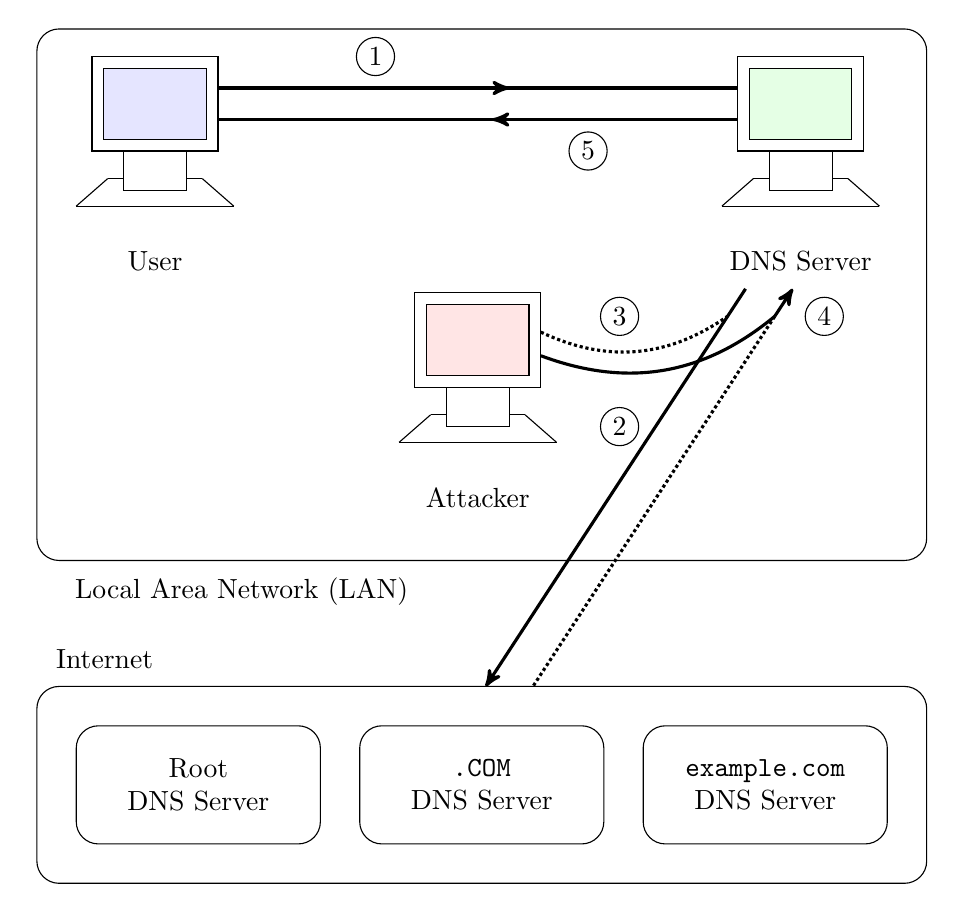
\begin{tikzpicture}
					\draw[fill=green!10] (3.05,2.15) rectangle (4.35,1.25);
					\draw (2.9,2.3) rectangle (4.5,1.1);
					\draw (4.1,1.1) rectangle (3.3,0.6);
					\draw (3.1,0.75) -- (2.7,0.4);
					\draw (4.3,0.75) -- (4.7,0.4);
					\draw (2.7,0.4) -- (4.7,0.4);
					\draw (3.1,0.75) -- (3.3,0.75);
					\draw (4.3,0.75) -- (4.1,0.75);
					\draw (3.7 ,-0.3) node[text width=3cm,align=center]{DNS Server};
					
					
					\draw[fill=blue!10] (-5.15,2.15) rectangle (-3.85,1.25);
					\draw (-5.3,2.3) rectangle (-3.7,1.1);
					\draw (-4.1,1.1) rectangle (-4.9,0.6);
					\draw (-5.1,0.75) -- (-5.5,0.4);
					\draw (-3.9,0.75) -- (-3.5,0.4);
					\draw (-5.5,0.4) -- (-3.5,0.4);
					\draw (-5.1,0.75) -- (-4.9,0.75);
					\draw (-3.9,0.75) -- (-4.1,0.75);
					\draw (-4.5,-0 .3) node[text width=3cm, align=center]{User};
					
						\draw[fill=red!10] (-1.05,-0.85) rectangle (0.25,-1.75);
					\draw (-1.2,-0.7) rectangle (0.4,-1.9);
					\draw (0,-1.9) rectangle (-0.8,-2.4);
					\draw (-1,-2.25) -- (-1.4,-2.6);
					\draw (0.2,-2.25) -- (0.6,-2.6);
					\draw (-1.4,-2.6) -- (0.6,-2.6);
					\draw (-1,-2.25) -- (-0.8,-2.25);
					\draw (0.2,-2.25) -- (0,-2.25);
					\draw (-0.4 ,-3.3) node[text width=3cm, align=center]{Attacker};
					
					\draw[rounded corners=8pt] (-6,2.65) rectangle (5.3,-4.1);
					
					\draw[<-,>=stealth',line width=0.4mm] (3.6,-0.65) -- (3.37, -1);
					\draw[densely dotted,line width=0.4mm] (3.37,-1) -- (0.3, -5.7);
					
					\draw[->,>=stealth',line width=0.4mm] (3,-0.65) -- (-0.3, -5.7);
					
					\draw[rounded corners=8pt] (-6,-5.7) rectangle (5.3,-8.2);
					
					\draw (-3.4,-4.5) node[align=left]{Local Area Network (LAN)};
					\draw (-5.14,-5.35) node[align=left]{Internet};
					
					\draw [rounded corners=8pt] (-5.5,-6.2) rectangle node[text width=3cm, align=center]{Root\\DNS Server} (-2.4, -7.7);
					\draw [rounded corners=8pt] (-1.9,-6.2) rectangle node[text width=3cm, align=center]{\texttt{.COM}\\DNS Server} (1.2, -7.7);
					\draw [rounded corners=8pt] (1.7,-6.2) rectangle node[text width=3cm, align=center]{\texttt{example.com}\\DNS Server} (4.8, -7.7);
					
					\draw[->,>=stealth',line width=0.4mm](-3.7,1.9) --(0,1.9);
					\draw[line width=0.4mm] (-0.3,1.9)--(2.9,1.9);
					\draw[-<,>=stealth',line width=0.4mm](-3.7,1.5) --(0,1.5);
					\draw[line width=0.4mm](-0.3,1.5) --(2.9,1.5);
					
					\draw[bend right, densely dotted, line width=0.4mm] (0.4,-1.2) to (2.77,-1);
					\draw[bend right, line width=0.4mm] (0.4,-1.5) to (3.37,-1);
					
				
					\draw (-1.7,2.3) node{\circled{1}};
					\draw (4,-1) node{\circled{4}};
					\draw (1,1.1) node{\circled{5}};
					\draw (1.4,-2.4) node {\circled{2}};
					\draw (1.4,-1) node {\circled{3}};
					\end{tikzpicture}
					
					\begin{flushleft}
					\circled{1} User's system sends out a DNS query to the DNS server.\\
					\circled{2} The DNS server will query other DNS servers over the internet if the records are not cached on the server.\\
					\circled{3} The attacker listens on the DNS request from the network and processes it.\\
					\circled{4} Before the DNS server over the internet is able to reply, the attacker sends out its own packet to spoof the DNS cache on the DNS server in the LAN.\\
					\circled{5} The spoofed information from the DNS server cache is sent back to the user's system to fulfil its DNS request.
					\end{flushleft}
					\centering
					
					\caption{Server DNS Spoofing}
					\label{fig:SpoofServRes}
				\end{figure}
\noindent \texttt{Netwox 105} is used again, but the filter switch is now changed to the IP address of the server instead (192.168.43.157).
\\\\To start this task, the cache must be flushed of any existing DNS requests. The following line does the required action.
\end{par}
\begin{verbatim}
$ sudo rndc flush
\end{verbatim}
\begin{par}
\noindent
The TTL is set to 3600 seconds (1 hour) to ensure that there is sufficient time to analyse the result as the DNS server will respond with the spoofed DNS request for the subsequent hour. The spoofing method will also be switched to \texttt{raw} as \texttt{netwox} will attempt to spoof the MAC address for the spoofed IP address, which is not required as \texttt{tool} will send an ARP request, which will take time to reply and may result in a failed attempt.
\end{par}
\begin{verbatim}
$ sudo netwox 105 --hostname "google.com" --hostnameip 5.6.7.8 
  --authns "google.com" --authnsip 192.168.43.157 --device "Eth0" 
  --ttl 3600 --filter "src host 192.168.43.157" --spoofip "raw"
\end{verbatim}
If the user's system is used to execute the command \texttt{dig google.com}, we will now see that the answer section reflects that the hostname is now redirected to IP address 5.6.7.8. Figure \ref{fig:cachepoison} shows that the answer section has been successfully modified.
\begin{figure}[H]
\centering
\includegraphics[width=0.7\linewidth]{cachepoison}
\caption{Google Hostname Redirect Query}
\label{fig:cachepoison}
\end{figure}
\noindent To also check that the DNS cache has been properly poisoned, the log files for the DNS cache is dumped into a plaintext database. The following code is executed to output the database.
\begin{verbatim}
$ sudo rndc dumpdb -cache
$ sudo cat /var/cache/bind/dump.db
\end{verbatim}
For simplicity, we do not print the entire database. Instead, the IP address for the \texttt{google.com} hostname is printed out only. As such, we use the following line instead.
\begin{verbatim}
$ sudo cat /var/cache/bind/dump.db | grep google.com
\end{verbatim}
Looking at the database dump in Figure \ref{fig:dbdump}, the A record reflects the same output as when the \texttt{dig} command has been executed on the user's computer as in Figure \ref{fig:cachepoison}. Furthermore, we notice that under the authority section in Figure \ref{fig:cachepoison}, the six digits represent the TTL for nameserver resolution (48 hours) and the only method of resolving this issue is to flush the DNS cache on the server and/or changing the DNS server to another IP address.
\begin{figure}[H]
\centering
\includegraphics[width=1\linewidth]{dbdump}
\caption{Google A Record}
\label{fig:dbdump}
\end{figure}
		\end{document}